\documentclass[11pt,a4paper]{report}
\usepackage[utf8]{inputenc}
\usepackage[T1]{fontenc}
\usepackage{amsmath,amssymb}
\usepackage{geometry}
\usepackage{enumitem}
\usepackage{parskip}
\usepackage{booktabs}
\usepackage{hyperref}
\usepackage{graphicx}
\usepackage{float}
\usepackage[table]{xcolor}
\usepackage{colortbl}
\usepackage{titlesec}
\usepackage{tcolorbox}
\usepackage{microtype}
\usepackage{mathpazo}
\usepackage{needspace}
\usepackage{framed}
\usepackage{subcaption}
\usepackage{longtable}
\tcbuselibrary{skins,breakable}

% ---- Color scheme (from Assignment-1 template) ----
\definecolor{sectionblue}{HTML}{1a365d}
\definecolor{subsectionblue}{HTML}{2c5282}
\definecolor{tableheader}{HTML}{e6f0f9}
\definecolor{titleaccent}{HTML}{2b6cb0}
\definecolor{LightGray}{HTML}{f7fafc}
\definecolor{TableZebra}{HTML}{edf2f7}

\geometry{
  a4paper,
  left=1.15in,
  right=1.15in,
  top=1.1in,
  bottom=1.1in,
}
\linespread{1.08}
\setlength{\parindent}{0pt}
\setlength{\parskip}{2.5pt plus 1pt}
\setlength{\emergencystretch}{1.5em}
\raggedbottom

% ---- Hyperref ----
\hypersetup{colorlinks=true, linkcolor=blue!70!black, urlcolor=blue!70!black, citecolor=blue!70!black}

% ---- Chapter: compact, section-like with rule ----
\titleformat{\chapter}[block]
  {\needspace{6\baselineskip}\normalfont\Large\bfseries\sffamily\color{sectionblue}}
  {\chaptertitlename\ \thechapter}{1em}{}
  [\color{sectionblue}\titlerule]
\titlespacing*{\chapter}{0pt}{1.5em}{0.8em}

% ---- Section ----
\titleformat{\section}
  {\needspace{5\baselineskip}\normalfont\Large\bfseries\sffamily\color{sectionblue}}
  {\thesection}{1em}{}
  [\color{sectionblue}\titlerule]
\titlespacing*{\section}{0pt}{1.5em}{0.8em}

% ---- Subsection ----
\titleformat{\subsection}
  {\needspace{4\baselineskip}\normalfont\large\bfseries\sffamily\color{subsectionblue}}
  {\thesubsection}{1em}{}
\titlespacing*{\subsection}{0pt}{1.2em}{0.5em}

% ---- Leftbar itemize (from Assignment-1 template) ----
\renewenvironment{leftbar}[1][\hsize]
  {\def\FrameCommand{{\color{subsectionblue}\vrule width 3pt}\hspace{0pt}}%
   \MakeFramed{\hsize#1\advance\hsize-\width\FrameRestore}}
  {\endMakeFramed}
\let\originalitemize\itemize
\let\endoriginalitemize\enditemize
\renewenvironment{itemize}{\begin{leftbar}\begin{originalitemize}}{\end{originalitemize}\end{leftbar}}

% ---- Caption ----
\usepackage{caption}
\captionsetup{labelfont=bf, font=small, skip=6pt}

\author{}
\date{}

\begin{document}
\begin{titlepage}
\centering
\vspace*{1.2cm}

\IfFileExists{iitb.eps}{\includegraphics[width=4cm]{iitb.eps}}{}

\vspace{1.2cm}

{\Large \textbf{Indian Institute of Technology Bombay} \par}

\vspace{0.4cm}
{\color{titleaccent}\rule{0.5\textwidth}{1.2pt}}
\vspace{1.2cm}

{\Huge \textbf{\color{sectionblue} Pre-trained CNN Representation Transfer} \par}
\vspace{0.4em}
{\Huge \textbf{\color{sectionblue} and Robustness Analysis} \par}

\vspace{1cm}

{\large \textbf{\color{subsectionblue} GNR 638} \\ Coding Assignment 2 \par}

\vspace{1.8cm}

{\large
\begin{tabular}{ll}
\textit{Authors:} & Indraneel Ghosh (24M0846)\\
                  & Sravani Gunnu (24M2116) \\
\end{tabular}
}

\vspace{0.8em}
{\normalsize \href{https://github.com/gunnusravani/GNR_638_Assignments}{github.com/gunnusravani/GNR\_638\_Assignments}}

\vfill

{\normalsize \color{subsectionblue} March 2026}

\end{titlepage}

\tableofcontents
\clearpage

%==============================================================================
\chapter{Introduction}
%==============================================================================

This report evaluates transferability, adaptation behavior, data efficiency, and robustness of ImageNet pre-trained CNN backbones on the AID 30-class aerial scene classification task.

The study answers the following assignment questions:
\begin{itemize}
  \item Which architecture transfers best and why?
  \item Which model is most robust under corruption?
  \item Which layers encode the most transferable semantics?
  \item When does fine-tuning improve or degrade robustness?
  \item How does parameter-efficiency relate to accuracy?
\end{itemize}

%==============================================================================
\chapter{Experimental Setup}
%==============================================================================

\section{Dataset}
\textbf{Dataset:} AID (30 classes) in ImageFolder format.\\
\textbf{Split:} \texttt{AID\_split/train}, \texttt{AID\_split/val}.\\
\textbf{Input resolution:} 299 for Inception-v3 compatibility (also used for ResNet50 and DenseNet121).

\section{Backbones}
\begin{itemize}
  \item ResNet50
  \item Inception-v3
  \item DenseNet121
\end{itemize}

\section{Training Configuration}
\begin{table}[H]
\centering
\caption{Global training configuration}
\label{tab:global-config}
\begin{tabular}{ll}
\toprule
\rowcolor{tableheader}
\textbf{Setting} & \textbf{Value} \\
\midrule
Optimizer & AdamW \\
Loss & Cross-Entropy \\
Batch size & 32 \\
Epochs & 30 \\
Learning rate & 1e-3 \\
Weight decay & 1e-4 \\
Seed & 1337 \\
Device & CUDA (fallback CPU) \\
\bottomrule
\end{tabular}
\end{table}

\section{Reproducibility and Artifact Paths}
\begin{itemize}
  \item Experiment command: \texttt{python run\_experiments.py}
  \item Results root: \texttt{results/linear\_probe/<backbone>/<timestamp>/}
  \item Checkpoints root: \texttt{model\_checkpoints/linear\_probe/<backbone>/<timestamp>/}
  \item Aggregated tables: \texttt{results/tables/}
  \item Commit hash: \texttt{<FILL\_COMMIT\_HASH>}
\end{itemize}

%==============================================================================
\chapter{Model Complexity and Efficiency}
%==============================================================================

For each backbone and transfer mode, we report parameter-efficiency statistics from the generated CSV tables.
\begin{itemize}
  \item Total parameters
  \item Trainable parameters
  \item MACs
  \item FLOPs
\end{itemize}

\begin{table}[H]
\centering
\caption{Model complexity summary}
\label{tab:model-complexity}
\begin{tabular}{llllll}
\toprule
\rowcolor{tableheader}
\textbf{Backbone} & \textbf{Transfer mode} & \textbf{Trainable params} & \textbf{Trainable frac} & \textbf{Val Acc} & \textbf{Acc / M trainable} \\
\midrule
ResNet50 & linear\_probe & 61,470 & 0.0026 & 0.8913 & 14.5003 \\
Inception-v3 & linear\_probe & 61,470 & 0.0028 & 0.8821 & 14.3501 \\
DenseNet121 & linear\_probe & 30,750 & 0.0044 & 0.9205 & 29.9335 \\
\bottomrule
\end{tabular}
\end{table}

%==============================================================================
\chapter{Scenario 1: Linear Probe Transfer}
%==============================================================================

\section{Objective}
Measure transferability when pre-trained backbones are used as frozen feature extractors.

\section{Implementation Details}
\begin{itemize}
  \item Freeze all backbone parameters.
  \item Replace final classification layer with a new linear layer for 30 classes.
  \item Train only the classifier head.
\end{itemize}

\section{Quantitative Summary}
\begin{table}[H]
\centering
\caption{Scenario 1 summary}
\label{tab:s1-summary}
\rowcolors{2}{TableZebra}{white}
\begin{tabular}{lccc}
\toprule
\rowcolor{tableheader}
\textbf{Backbone} & \textbf{Best Val Acc} & \textbf{Macro F1} & \textbf{Checkpoint} \\
\midrule
ResNet50 & 0.8913 & 0.8847 & best.pt \\
Inception-v3 & 0.8821 & 0.8750 & best.pt \\
DenseNet121 & 0.9205 & 0.9155 & best.pt \\
\bottomrule
\end{tabular}
\end{table}

\vspace{-0.4em}
\begin{center}
\small
ResNet50: best val acc = 0.8913, macro F1 = 0.8847.\
\end{center}

\section{Accuracy Curves}
\begin{figure}[H]
  \centering
  \begin{subfigure}{0.32\textwidth}
    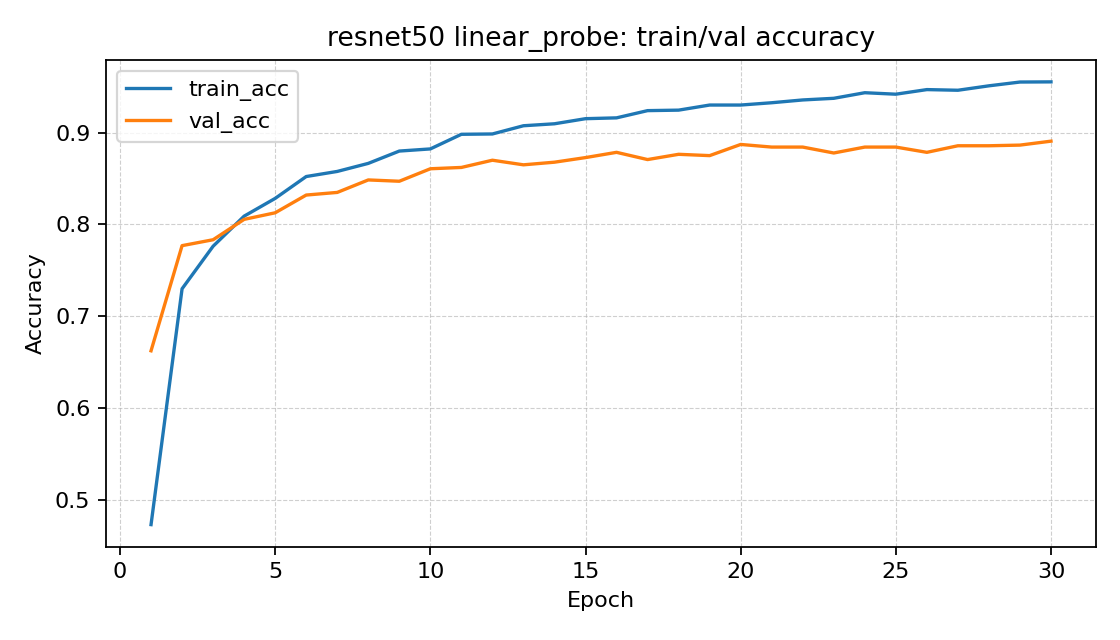
\includegraphics[width=\linewidth]{results/linear_probe/resnet50/20260313-114331/accuracy_curves.png}
    \caption{ResNet50}
  \end{subfigure}
  \begin{subfigure}{0.32\textwidth}
    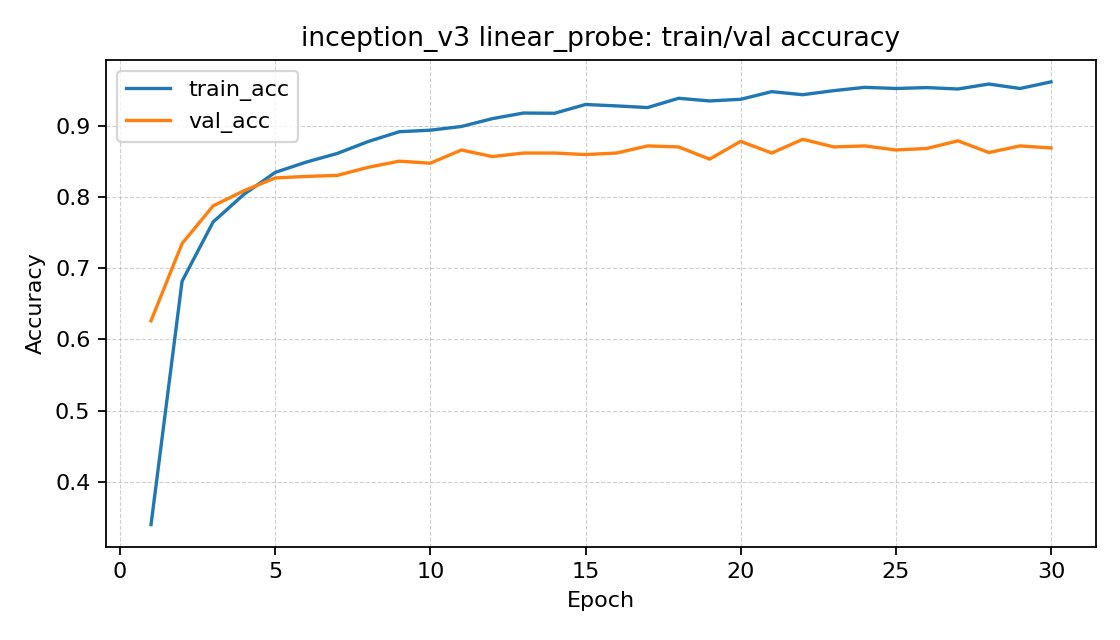
\includegraphics[width=\linewidth]{results/linear_probe/inception_v3/20260313-115321/accuracy_curves.png}
    \caption{Inception-v3}
  \end{subfigure}
  \begin{subfigure}{0.32\textwidth}
    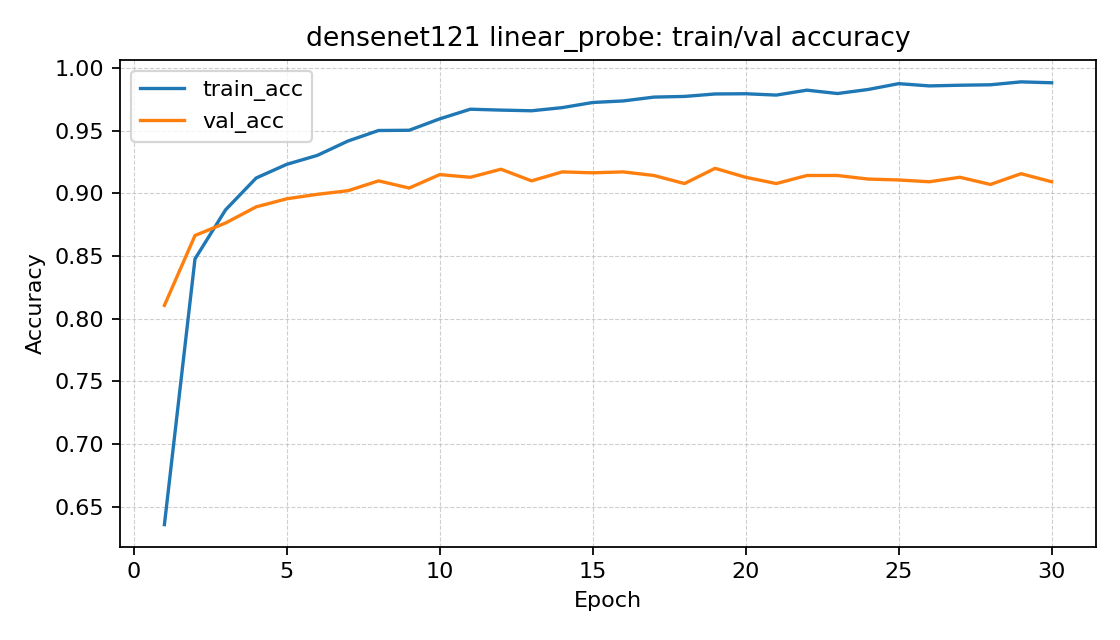
\includegraphics[width=\linewidth]{results/linear_probe/densenet121/20260313-120249/accuracy_curves.png}
    \caption{DenseNet121}
  \end{subfigure}
  \caption{Training and validation accuracy curves under linear probing.}
  \label{fig:s1-acc}
\end{figure}

\section{Confusion Matrices}
\begin{figure}[H]
  \centering
  \begin{subfigure}{0.32\textwidth}
    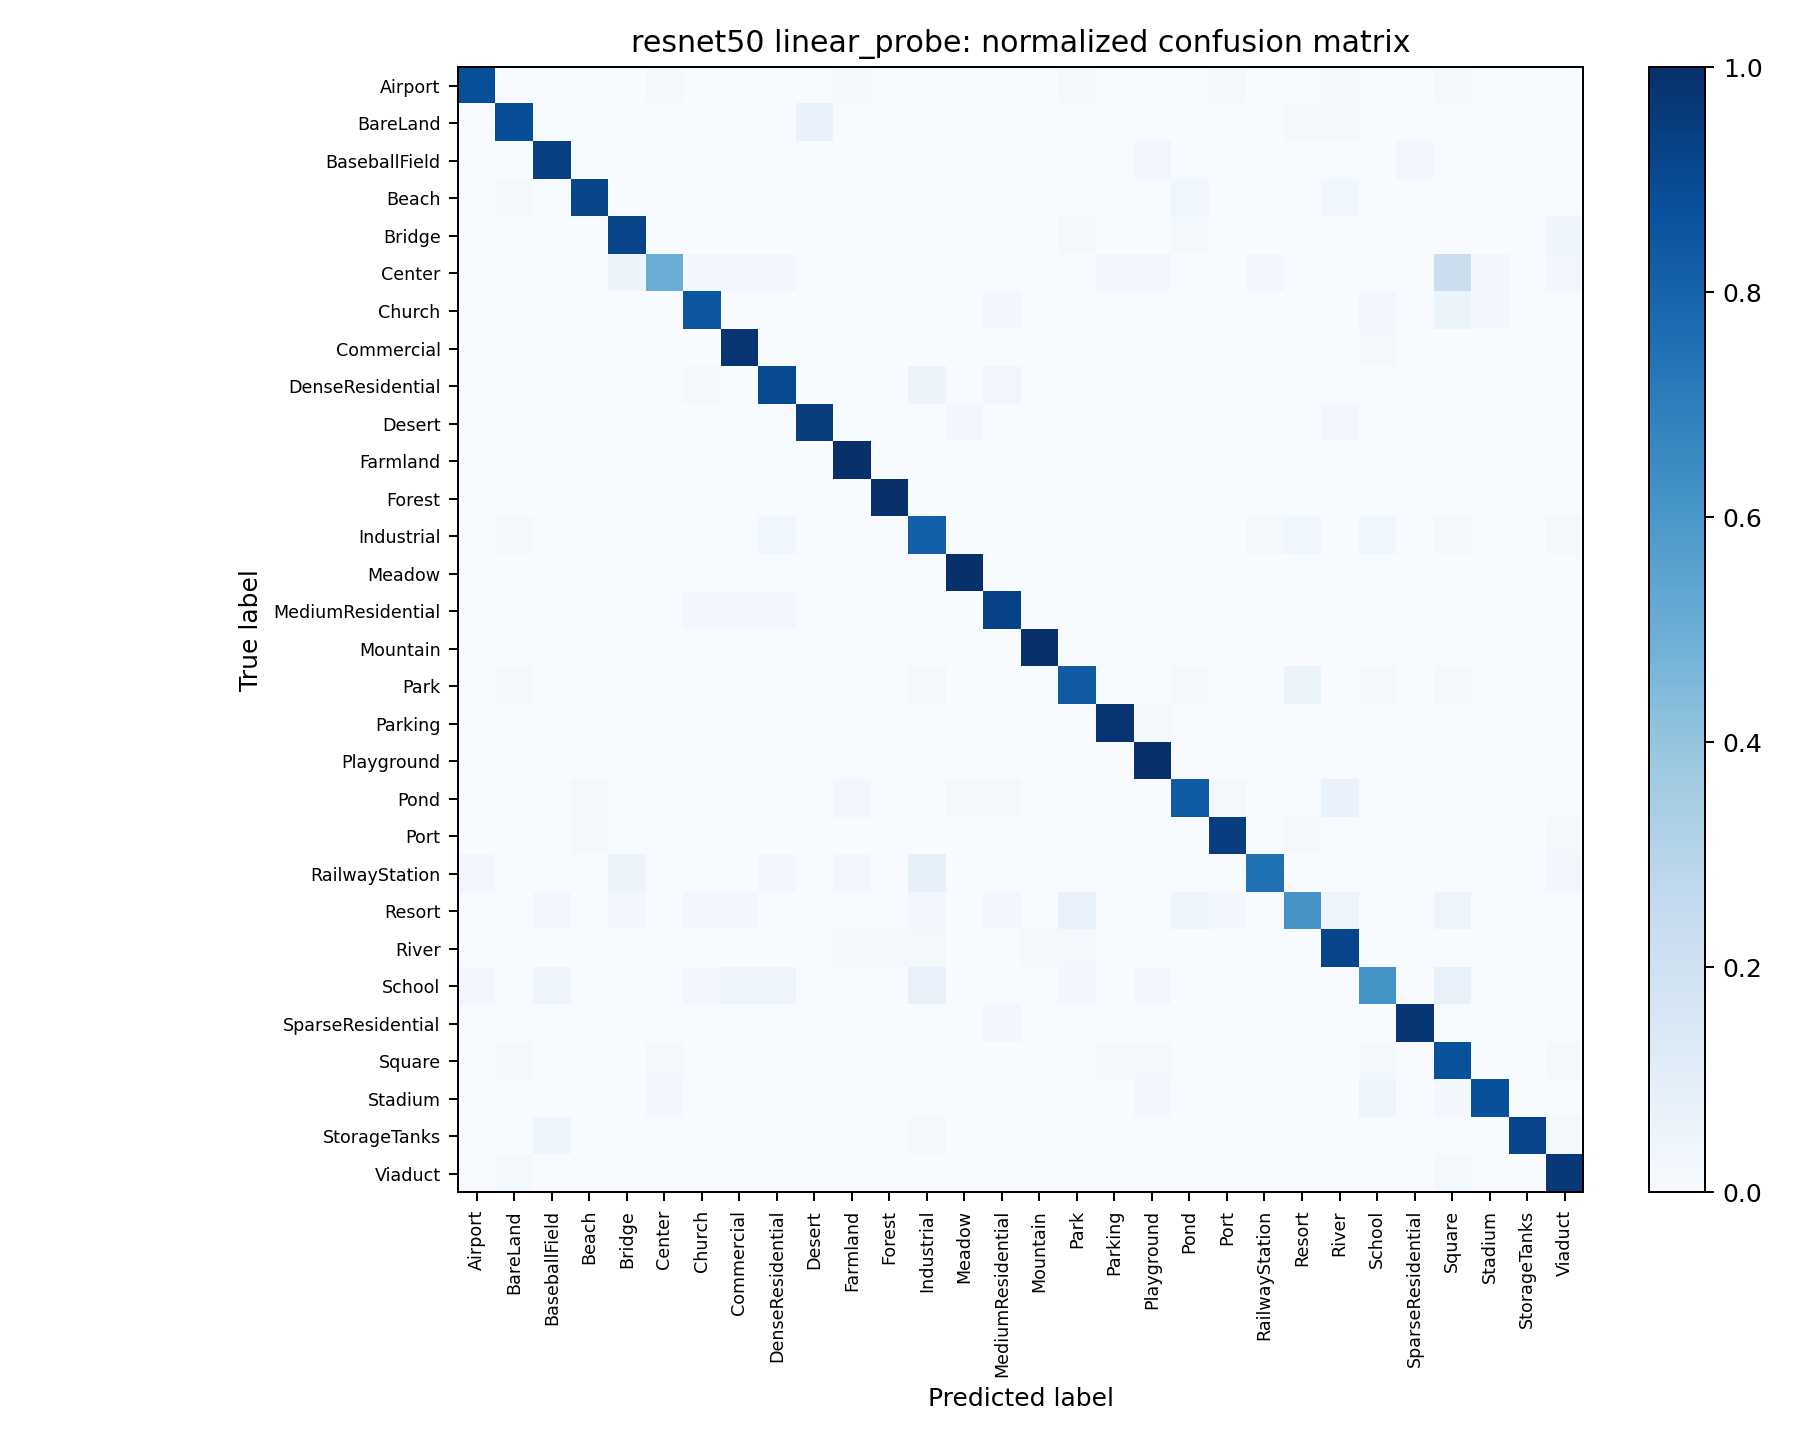
\includegraphics[width=\linewidth]{results/linear_probe/resnet50/20260313-114331/confusion_matrix.png}
    \caption{ResNet50}
  \end{subfigure}
  \begin{subfigure}{0.32\textwidth}
    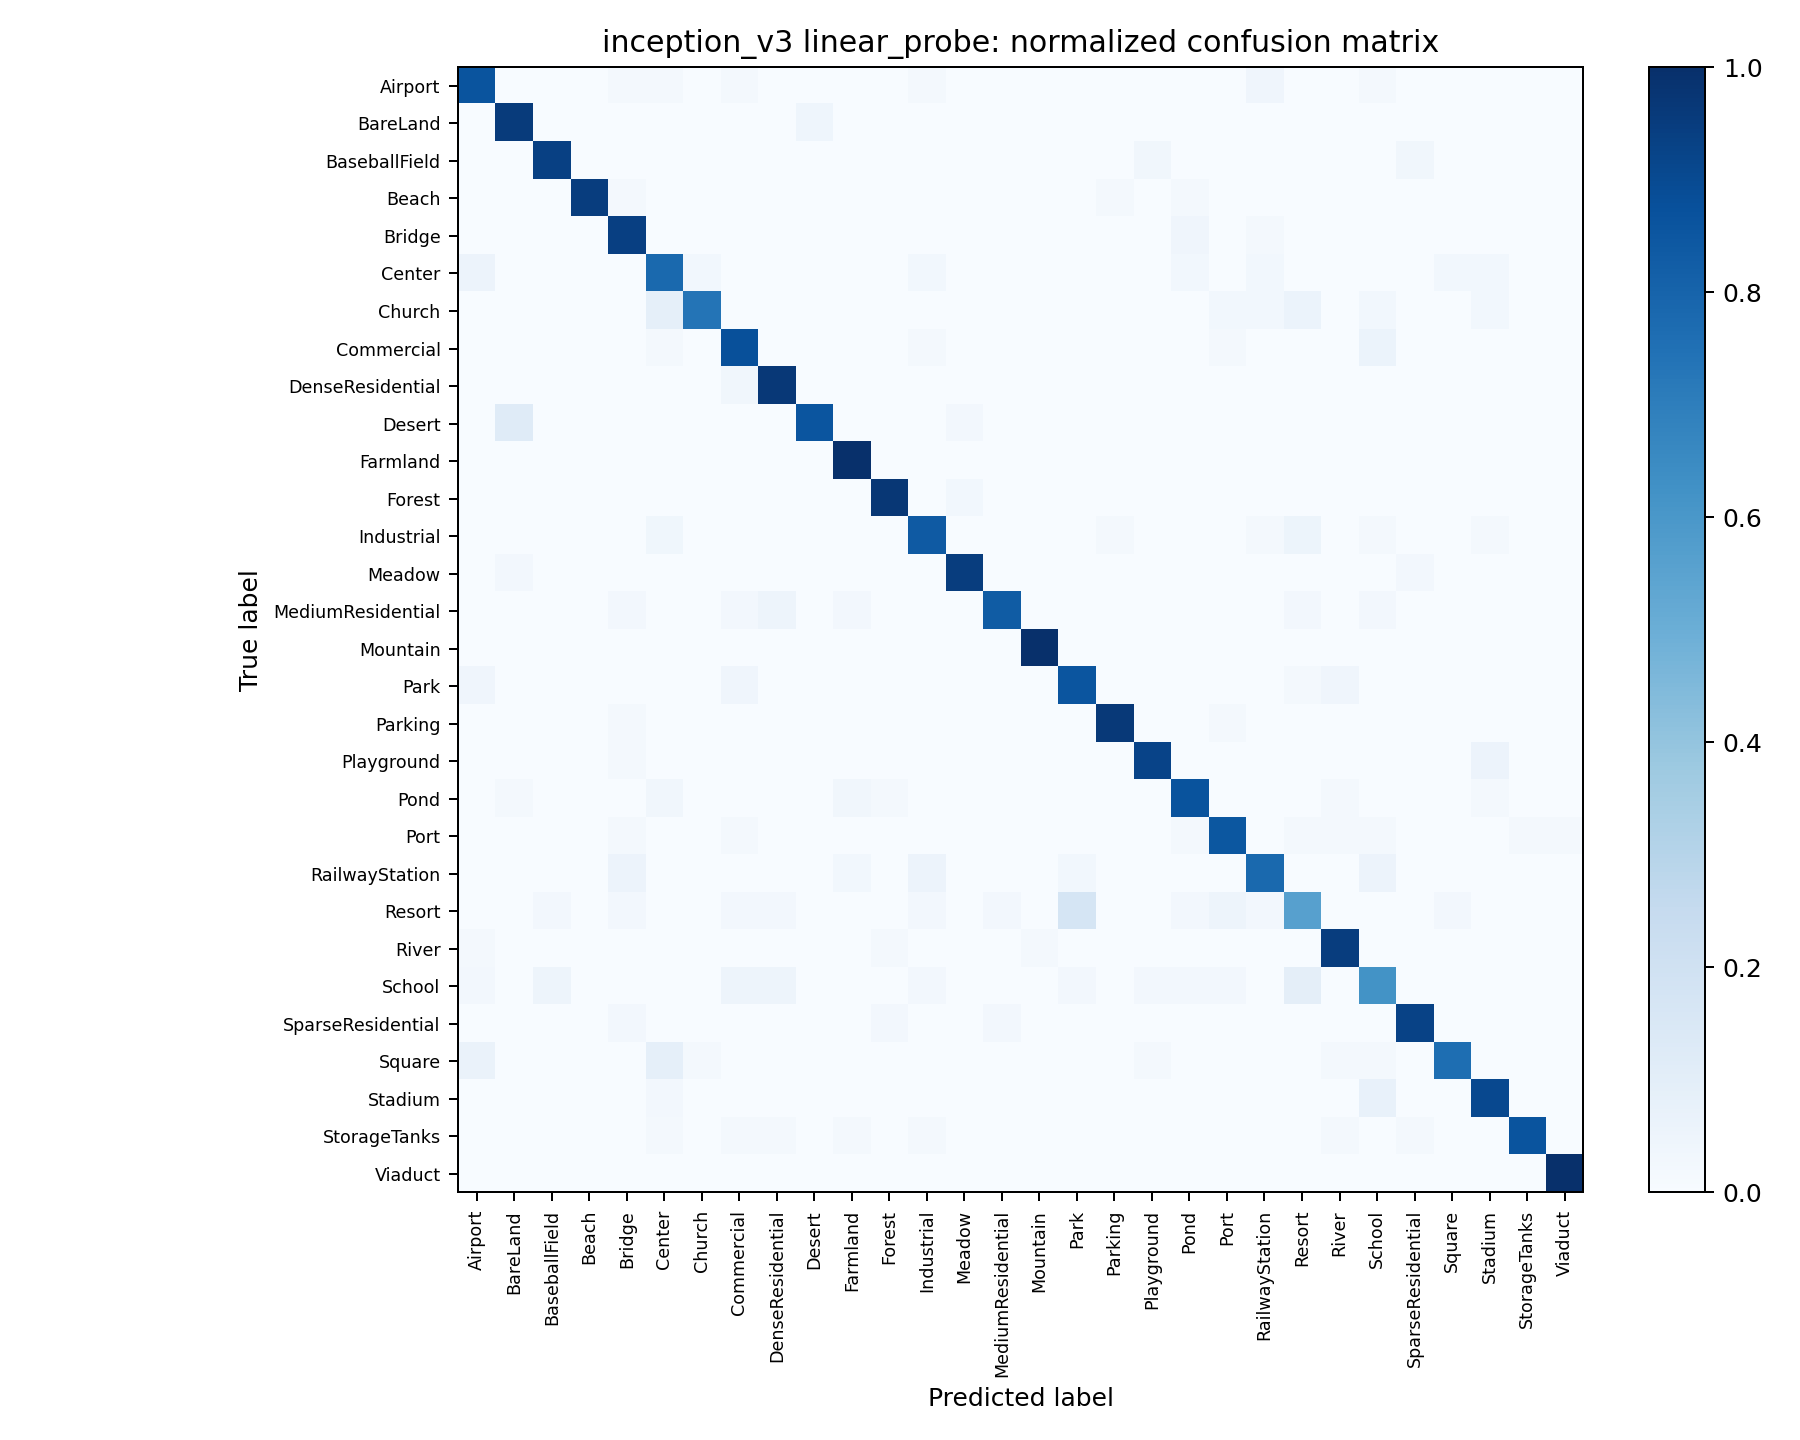
\includegraphics[width=\linewidth]{results/linear_probe/inception_v3/20260313-115321/confusion_matrix.png}
    \caption{Inception-v3}
  \end{subfigure}
  \begin{subfigure}{0.32\textwidth}
    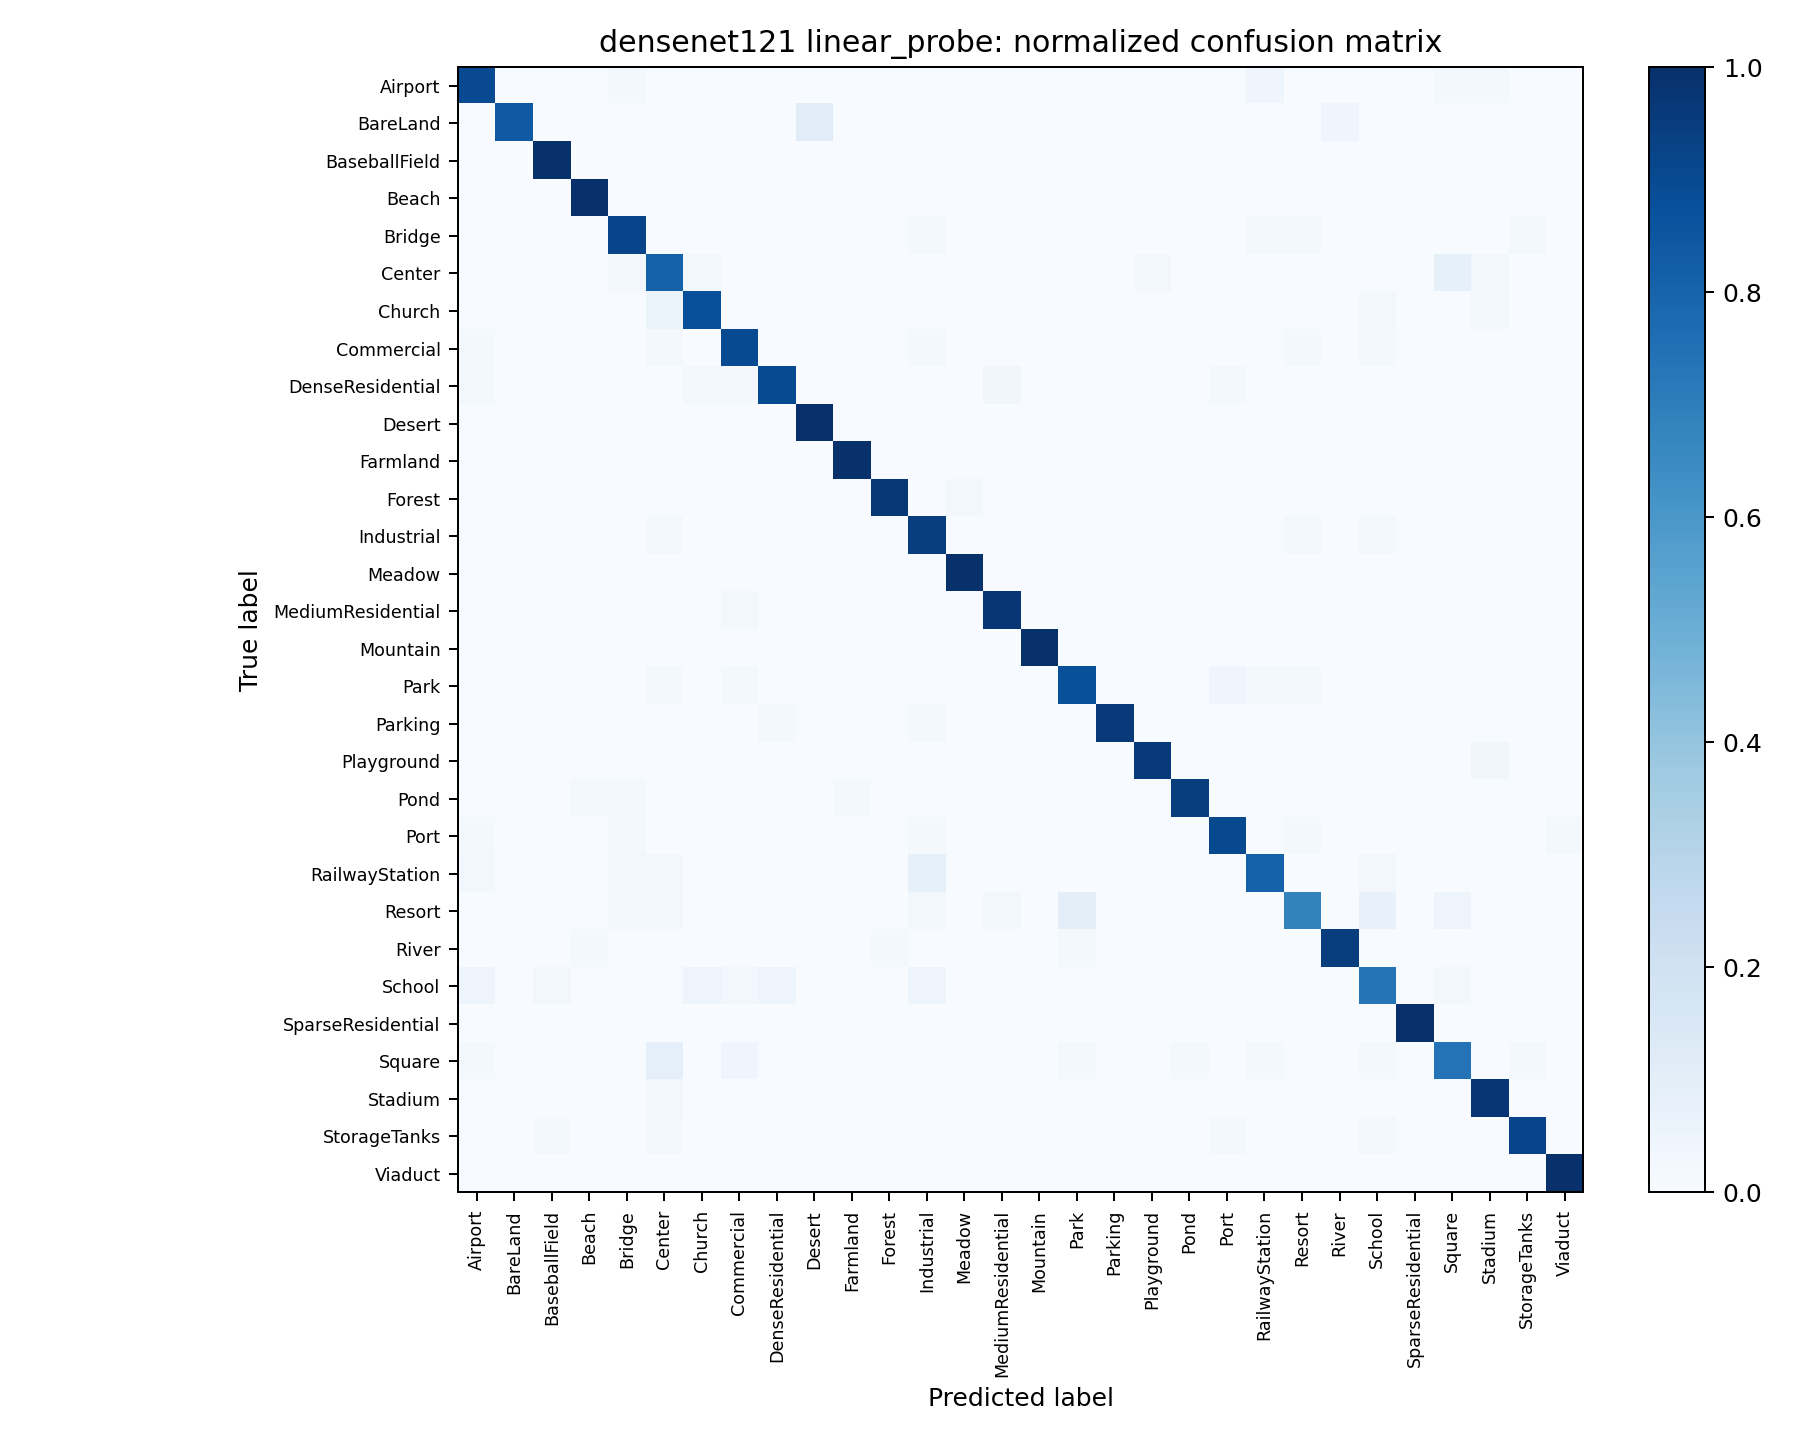
\includegraphics[width=\linewidth]{results/linear_probe/densenet121/20260313-120249/confusion_matrix.png}
    \caption{DenseNet121}
  \end{subfigure}
  \caption{Normalized confusion matrices for Scenario 1.}
  \label{fig:s1-cm}
\end{figure}

\section{Feature Embeddings (PCA and t-SNE)}
\begin{figure}[H]
  \centering
  \begin{subfigure}{0.32\textwidth}
    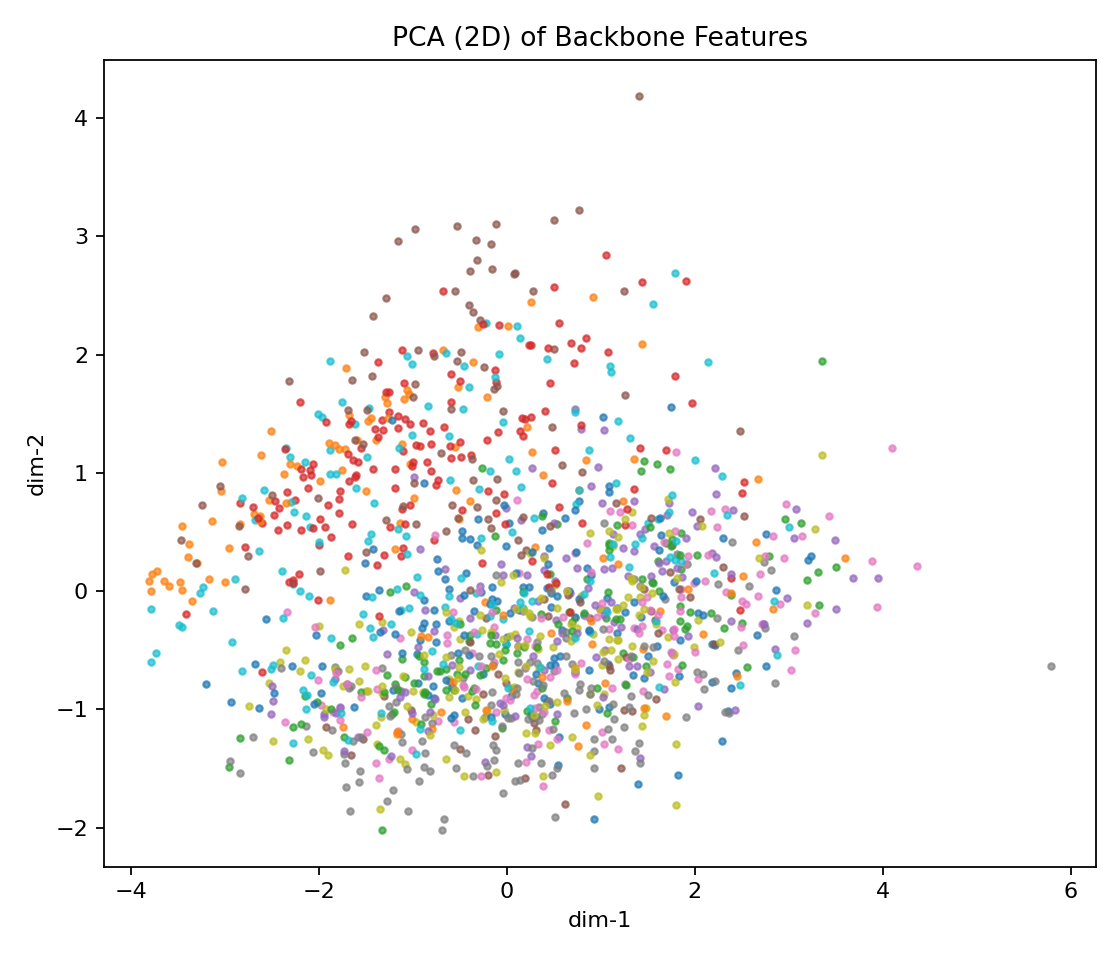
\includegraphics[width=\linewidth]{results/linear_probe/resnet50/20260313-114331/feature_viz/pca_2d.png}
    \caption{ResNet50 PCA}
  \end{subfigure}
  \begin{subfigure}{0.32\textwidth}
    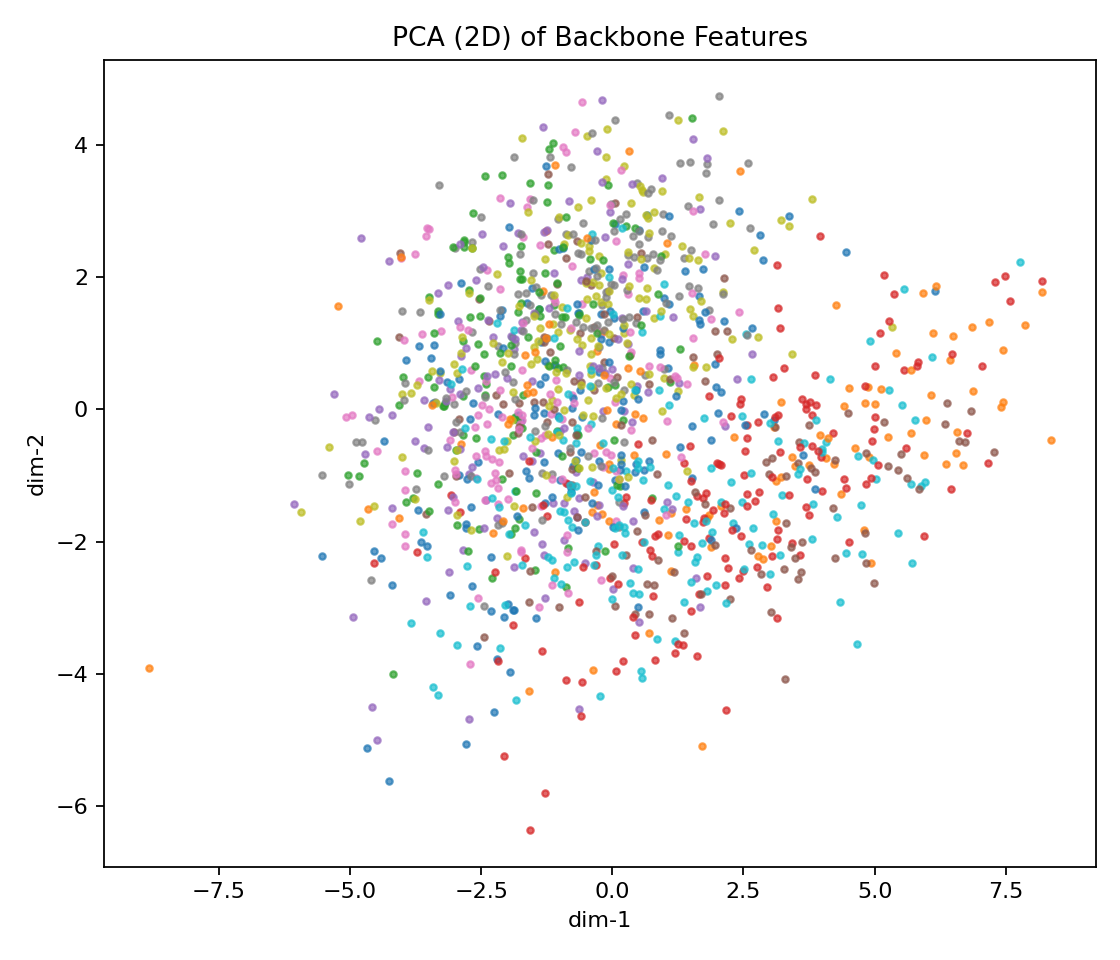
\includegraphics[width=\linewidth]{results/linear_probe/inception_v3/20260313-115321/feature_viz/pca_2d.png}
    \caption{Inception-v3 PCA}
  \end{subfigure}
  \begin{subfigure}{0.32\textwidth}
    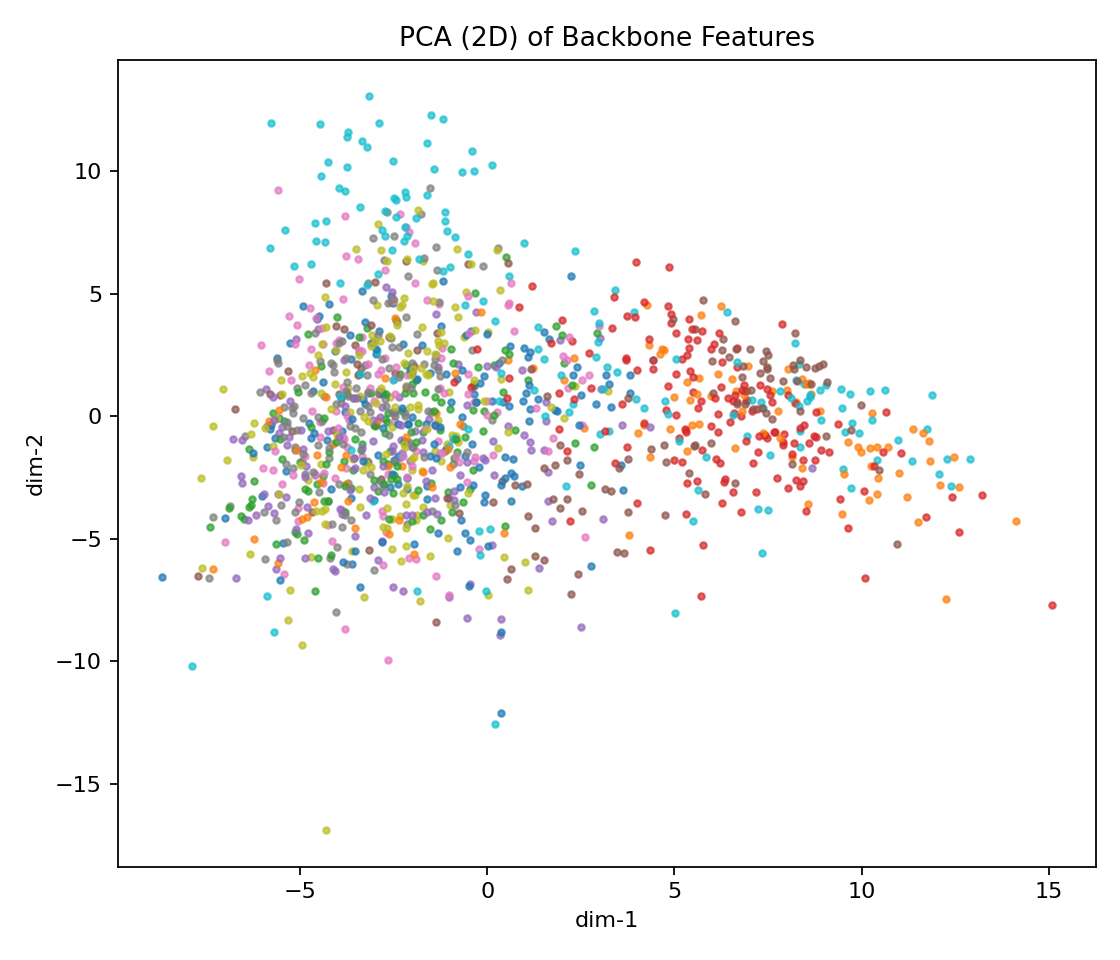
\includegraphics[width=\linewidth]{results/linear_probe/densenet121/20260313-120249/feature_viz/pca_2d.png}
    \caption{DenseNet121 PCA}
  \end{subfigure}
  \caption{PCA feature visualizations.}
  \label{fig:s1-pca}
\end{figure}

\begin{figure}[H]
  \centering
  \begin{subfigure}{0.32\textwidth}
    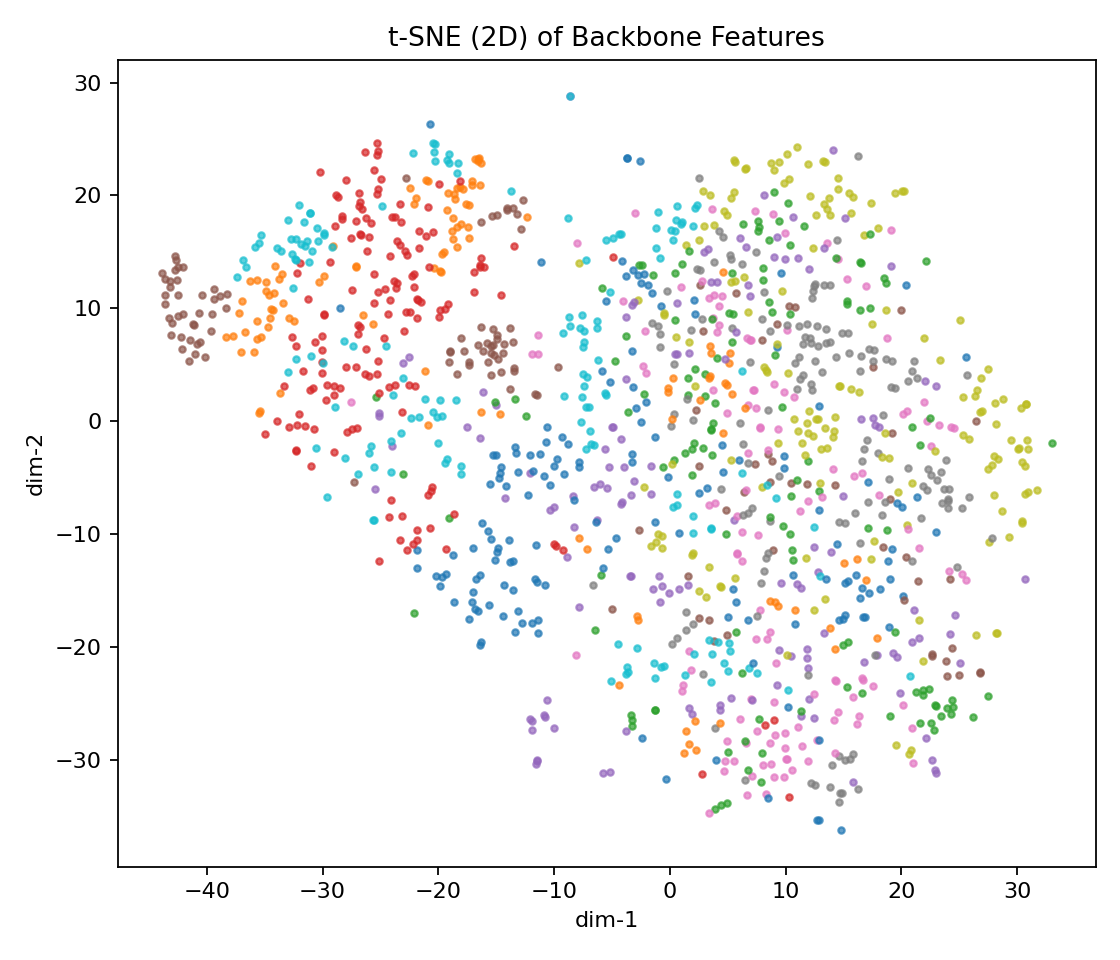
\includegraphics[width=\linewidth]{results/linear_probe/resnet50/20260313-114331/feature_viz/tsne_2d.png}
    \caption{ResNet50 t-SNE}
  \end{subfigure}
  \begin{subfigure}{0.32\textwidth}
    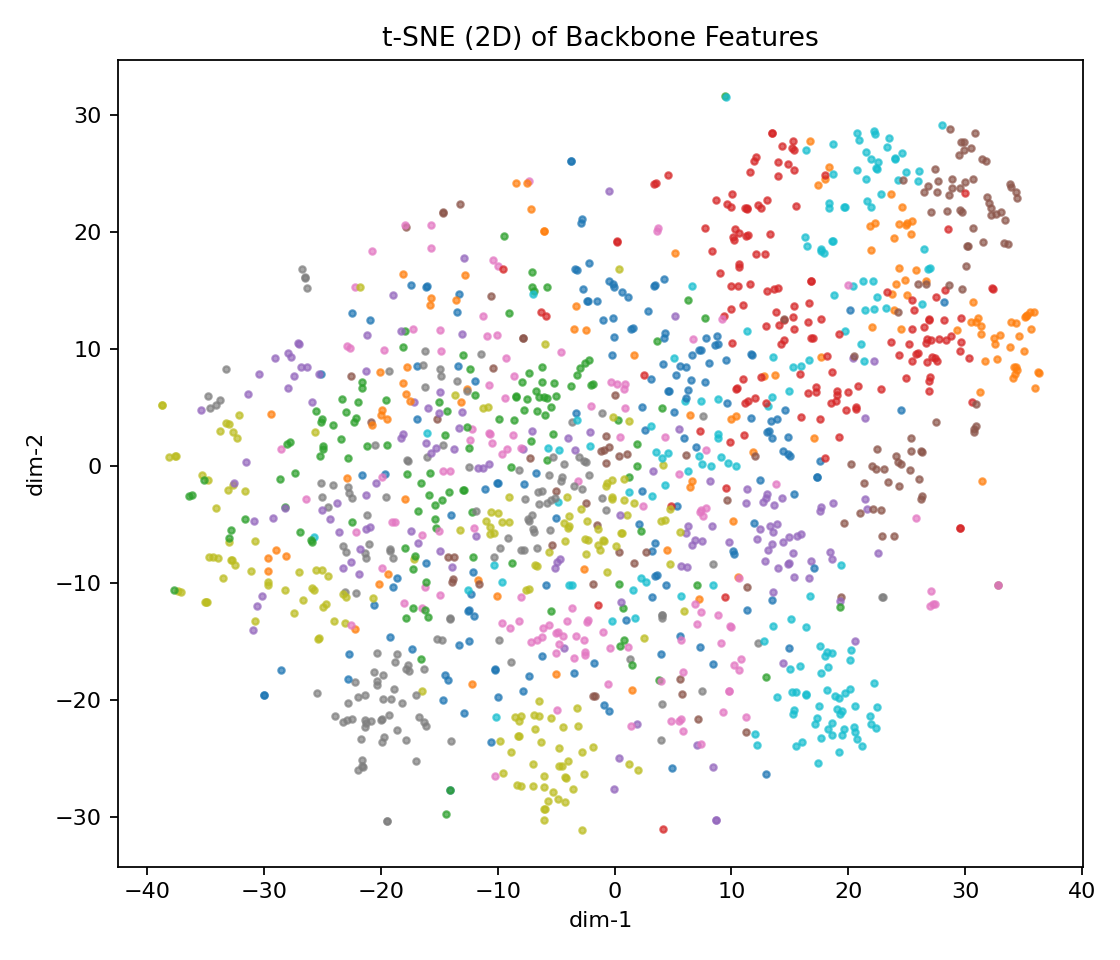
\includegraphics[width=\linewidth]{results/linear_probe/inception_v3/20260313-115321/feature_viz/tsne_2d.png}
    \caption{Inception-v3 t-SNE}
  \end{subfigure}
  \begin{subfigure}{0.32\textwidth}
    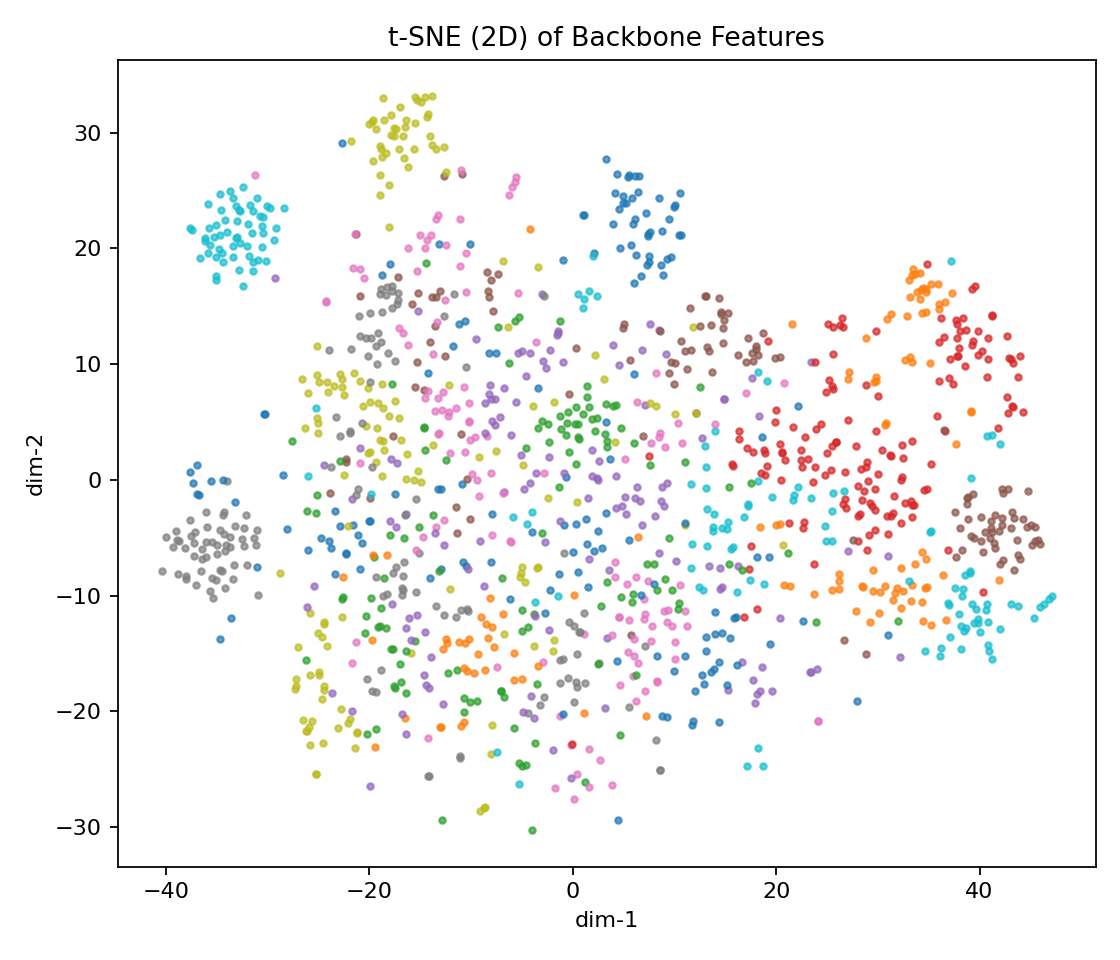
\includegraphics[width=\linewidth]{results/linear_probe/densenet121/20260313-120249/feature_viz/tsne_2d.png}
    \caption{DenseNet121 t-SNE}
  \end{subfigure}
  \caption{t-SNE feature visualizations.}
  \label{fig:s1-tsne}
\end{figure}

\section{Discussion}
\textbf{Separability:} All three backbones show strong class structure, with t-SNE exhibiting better local clustering than PCA. DenseNet121 shows comparatively tighter cluster compactness for several classes, matching its stronger macro metrics.\\
\textbf{Transfer quality:} DenseNet121 achieved the best linear-probe performance (val acc 0.9205, macro F1 0.9155), followed by ResNet50 (0.8913, 0.8847), then Inception-v3 (0.8821, 0.8750). Training curves indicate rapid early convergence for all models and stable validation after approximately 10 epochs.\\
\textbf{Failure cases:} Confusion matrices suggest persistent confusion among visually similar urban classes (for example, residential/commercial categories), indicating that frozen backbones still retain some class-overlap under domain-specific aerial textures.

%==============================================================================
\chapter{Scenario 2: Fine-Tuning Strategies}
%==============================================================================

\section{Objective}
Compare linear probe, last-block fine-tuning, full fine-tuning, and selective 20\% unfreezing under fixed hyperparameters.

\section{Required Outputs}
\begin{itemize}
  \item Validation accuracy vs trainable parameter percentage.
  \item Gradient norm statistics across layers.
  \item Convergence stability (training loss vs epoch).
\end{itemize}

\begin{table}[H]
\centering
\caption{Fine-tuning strategy comparison}
\label{tab:s2}
\begin{tabular}{llllll}
\toprule
\rowcolor{tableheader}
\textbf{Backbone} & \textbf{Strategy} & \textbf{Trainable \%} & \textbf{Best Val Acc} & \textbf{Final Train Loss} & \textbf{Notes} \\
\midrule
<fill> & <fill> & <fill> & <fill> & <fill> & <fill> \\
\bottomrule
\end{tabular}
\end{table}

%==============================================================================
\chapter{Scenario 3: Few-Shot Learning Analysis}
%==============================================================================

\section{Objective}
Evaluate data efficiency at 100\%, 20\%, and 5\% training data.

\section{Metrics}
Relative performance drop:
\begin{equation}
\Delta = \frac{\mathrm{Acc}_{100\%} - \mathrm{Acc}_{5\%}}{\mathrm{Acc}_{100\%}}
\end{equation}

Training-validation gap:
\begin{equation}
\mathrm{Gap} = \mathrm{Acc}_{\mathrm{train}} - \mathrm{Acc}_{\mathrm{val}}
\end{equation}

\begin{table}[H]
\centering
\caption{Few-shot summary}
\label{tab:s3}
\begin{tabular}{llllll}
\toprule
\rowcolor{tableheader}
\textbf{Backbone} & \textbf{Acc@100\%} & \textbf{Acc@20\%} & \textbf{Acc@5\%} & \textbf{$\Delta$} & \textbf{Gap} \\
\midrule
<fill> & <fill> & <fill> & <fill> & <fill> & <fill> \\
\bottomrule
\end{tabular}
\end{table}

%==============================================================================
\chapter{Scenario 4: Corruption Robustness Evaluation}
%==============================================================================

\section{Objective}
Compare clean-vs-corrupted accuracy under Gaussian noise, motion blur, and brightness shift.

\section{Metrics}
Corruption error:
\begin{equation}
\mathrm{Corruption\ Error} = 1 - \mathrm{Acc}_{\mathrm{corrupted}}
\end{equation}

Relative robustness:
\begin{equation}
\mathrm{Relative\ Robustness} = \frac{\mathrm{Acc}_{\mathrm{corrupted}}}{\mathrm{Acc}_{\mathrm{clean}}}
\end{equation}

\begin{table}[H]
\centering
\caption{Robustness summary}
\label{tab:s4}
\begin{tabular}{lllllll}
\toprule
\rowcolor{tableheader}
\textbf{Backbone} & \textbf{Clean Acc} & \textbf{Mean Corr Acc} & \textbf{Worst Corr Acc} & \textbf{Mean Drop} & \textbf{Worst Drop} & \textbf{Notes} \\
\midrule
<fill> & <fill> & <fill> & <fill> & <fill> & <fill> & <fill> \\
\bottomrule
\end{tabular}
\end{table}

%==============================================================================
\chapter{Scenario 5: Layer-Wise Feature Probing}
%==============================================================================

\section{Objective}
Analyze feature quality at early, middle, and final layers.

\section{Required Outputs}
\begin{itemize}
  \item Validation accuracy vs depth.
  \item Feature norm statistics by depth.
  \item PCA 2D on a fixed subset (30 classes, 30 samples per class) across all models/layers.
\end{itemize}

\begin{table}[H]
\centering
\caption{Layer-wise probing summary}
\label{tab:s5}
\begin{tabular}{llllll}
\toprule
\rowcolor{tableheader}
\textbf{Backbone} & \textbf{Acc (early)} & \textbf{Acc (mid)} & \textbf{Acc (final)} & \textbf{Norm trend} & \textbf{Interpretation} \\
\midrule
<fill> & <fill> & <fill> & <fill> & <fill> & <fill> \\
\bottomrule
\end{tabular}
\end{table}

%==============================================================================
\chapter{Cross-Scenario Analysis}
%==============================================================================

\section{Accuracy and Efficiency Trade-offs}
Use generated tables in \texttt{results/tables/}: accuracy comparison, robustness comparison, and parameter efficiency.

\section{Unexpected Finding}
<fill>

\section{Negative/Failure Case}
<fill>

%==============================================================================
\chapter{Computational Budget}
%==============================================================================

\begin{table}[H]
\centering
\caption{Compute budget summary}
\label{tab:budget}
\begin{tabular}{lllll}
\toprule
\rowcolor{tableheader}
\textbf{Scenario} & \textbf{Backbone} & \textbf{Epochs} & \textbf{Runtime (hh:mm)} & \textbf{Hardware} \\
\midrule
Scenario 1 & ResNet50 & 30 & 00:09:38 & <FILL\_HARDWARE> \\
Scenario 1 & Inception-v3 & 30 & 00:09:14 & <FILL\_HARDWARE> \\
Scenario 1 & DenseNet121 & 30 & 00:09:27 & <FILL\_HARDWARE> \\
\bottomrule
\end{tabular}
\end{table}

%==============================================================================
\chapter{Conclusions}
%==============================================================================

\begin{itemize}
  \item Best transfer architecture and rationale.
  \item Most robust architecture and corruption sensitivity pattern.
  \item Most transferable depth and semantic abstraction trend.
  \item Fine-tuning conditions that improve/degrade robustness.
  \item Parameter-efficiency insights.
\end{itemize}

\begin{tcolorbox}[
  colback=LightGray,
  colframe=black!40,
  boxrule=0.6pt,
  arc=2pt,
  left=4pt,
  right=4pt,
  top=6pt,
  bottom=6pt,
  breakable=false,
  title=\textbf{Final Summary},
  coltitle=black,
  colbacktitle=LightGray,
  fonttitle=\bfseries,
]
\color{black}%
<Write your concise final takeaway here after all five scenarios are complete.>
\end{tcolorbox}

\appendix
\chapter{Commands and File Mapping}

\section{Commands}
\begin{verbatim}
python train.py
python evaluate.py --ckpt <path_to_ckpt> --robust --linear-probe-depths
python run_experiments.py
\end{verbatim}

\section{Scenario-1 Artifact Mapping}
\begin{itemize}
  \item Accuracy curves: \texttt{results/linear\_probe/<backbone>/<timestamp>/accuracy_curves.png}
  \item Confusion matrix: \texttt{results/linear\_probe/<backbone>/<timestamp>/confusion_matrix.png}
  \item Classification report: \texttt{results/linear\_probe/<backbone>/<timestamp>/classification_report.txt}
  \item PCA/t-SNE: \texttt{results/linear\_probe/<backbone>/<timestamp>/feature\_viz/}
  \item Checkpoints: \texttt{model\_checkpoints/linear\_probe/<backbone>/<timestamp>/(best.pt, latest.pt)}
\end{itemize}

\end{document}
